\documentclass[11pt]{article}
\usepackage{amsmath, amssymb}
\usepackage{geometry}
\geometry{margin=1in}
\usepackage{fancyhdr}
\usepackage{lastpage}
\usepackage{parskip} % Better paragraph spacing
\usepackage{titlesec} % Better section formatting
\usepackage{graphicx}
\usepackage{float}
\usepackage[most]{tcolorbox}
\usepackage{lmodern}
\usepackage{caption}

% Define commands for reusable content
\newcommand{\coursename}{COM-402 Information Security Privacy}
\newcommand{\lecturenum}{04}
\newcommand{\lecturedate}{\today}
\newcommand{\professor}{Mathias Payer}

% Configure section spacing
\titlespacing*{\section}{0pt}{2ex plus 1ex minus .2ex}{1.5ex plus .2ex}
% Header / Footer
\pagestyle{fancy}
\fancyhf{}
\fancyhead[L]{\coursename}
\fancyhead[R]{Lecture \lecturenum}
\fancyfoot[L]{EPFL - Computer Science}
\fancyfoot[C]{Author: Jonathan Dutoit}
\fancyfoot[R]{Page \thepage\ of \pageref{LastPage}}

\begin{document}

\begin{center}
  {\large EPFL - Computer Science} \\[0.5em]
  {\Large \textbf{\coursename}} \\[0.5em]
  {\large Lecture \lecturenum\ --- \lecturedate} \\[0.5em]
  {\large Author: Jonathan Dugout} \\[0.5em]
  {\large Professor: \professor} \\[0.5em]
\end{center}

\vspace{2cm}

\begin{center}
	{\LARGE \textbf{Data Security}}
\end{center}

\vspace{1cm}

\section*{Learning Goals}
\begin{itemize}
	\item Understand how access control and encryption are applied in data security
	\item Learn methods of secure password storage and techniques for password cracking
	\item Know the basic of Secure Remote Password Protocol (SRP)
\end{itemize}

\section*{Data Security}
Data storage requirements are ubiquitous 
\begin{itemize}
	\item Banking, industry, social networks, government, research, or mobile apps
	\item Leads to new types of analysis (big data, machine learning)
\end{itemize}

Companies must consider security of data they store
\begin{itemize}
	\item What are security requirements of DB systems?
	\item What are the main attack vectors of DB systems?
	\item What are main protections of DB systems?
\end{itemize}

\section*{Typical Setups}
\begin{itemize}
	\item Client $\Rightarrow$ Internet $\Leftrightarrow$ Firewall $\Leftrightarrow$ Web server farm $\Leftrightarrow$ Database
		\begin{itemize}
			\item On premises
		\end{itemize}
	\item Client $\Rightarrow$ Internet $\Leftrightarrow$ Website instances  $\Leftrightarrow$ Database
		 \begin{itemize}
			\item In the cloud / PaaS (patform-as-a-service)
		\end{itemize}
\end{itemize}

\section*{Multitier Architecture}

\begin{itemize}
	\item 1) Presentation tier (user interface, web pages, static content). The top-most level of the application. The main function of the interface is to translate tasks and results to something that is intuitive.
	\item 2) Application (logic) tier. This layer coordinates the application, processes commands, makes logical decisions and evaluations, and performs calculations. It also moves and processes data between the two surrounding layers.
	\item 3) Data tier (provides data persistence and APIs to access data). Here the information is stored and retrieved from a database or file system. The information is then passed back to the logic tier for processing, and then eventually back to the user.
\end{itemize}

\section*{Examples of DB Attacks}
\begin{itemize}
	\item Washington state
	\item Amadeus IT group
	\item Epic Games (2019-01). All Fortnite player accounts accessible exposing credit card info etc.
	\item Steam (2018-11) API vulnerability gave access to CD keys for any game. Now patched
\end{itemize}

\vspace{0.5cm}

\begin{center}
  {\LARGE \textbf{Database: Access Control}}
\end{center}

\vspace{0.5cm}

\section*{Layers of database}

The layers of database accesses:
% Quick centered image
\begin{figure}[H]
    \centering
    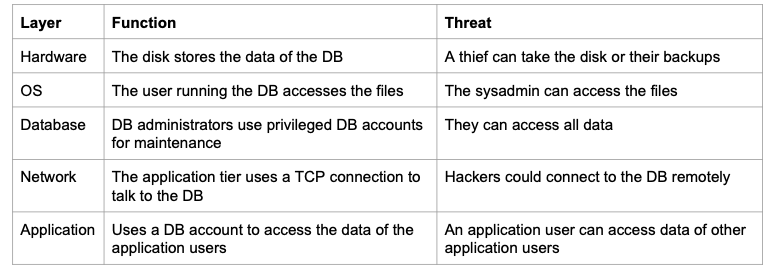
\includegraphics[width=0.8\textwidth]{database-layers}
    \label{fig:LABEL}
\end{figure}
\begin{tcolorbox}[
  colback=orange!15,     % background color
  colframe=black!50,    % border color
  boxrule=1pt,       % border thickness
  arc=3mm,             % rounded corners
  left=4mm, right=4mm, top=2mm, bottom=2mm % padding
]
Each layer needs to implement proper access control!
\end{tcolorbox}

\section*{Access Control: Least Privilege}

Access control defines which actor can access which resource. 

We should apply the principle of \textbf{least privilege}

\begin{itemize}
	\item Each actor can only access the resources strictly needed for its function
\end{itemize}

This must be applied across all levels of the DB

\section*{Hardware Access Control}
If it is a physical machine in a data center

\begin{itemize}
	\item Physical protection: locks, cameras, alarms
\end{itemize}

If it is a virtual machine in the cloud
\begin{itemize}
	\item Cloning the machine is like stealing the hard disk
	\item Limit the number of people who have the right to clone
	\item Use strong authentication for your cloud management console (e.g., 2FA)
\end{itemize}

\section*{OS Access Control}
The DB runs as a process in the OS, owned by a certain OS user (e.g., mysql, oracle)

This user is the only one allowed to access the files of the database. 

Only user mysql is alloed to access this directory, or any user with root privileges!

\section*{Discretionary DB Access Control}

SQL databases use \textbf{discretionary} access control (DAC) to grant user access to objects (table and view) through privileges (SELECT, INSERT, UPDATE, DELETE, CREATE, DROP)

By default, the \verb|root| or \verb|system| user has all privileges on all objects.

\section*{Role-Based DB Access Control}

SQL databases also support \textcolor{red}{role based} access control

Roles are created very much like users
\begin{itemize}
	\item Privileges can be granted to roles
	\item Then, roles can be granted to users
\end{itemize}

E.g., profs can read most columns but only change grades.

You can grant several roles to a same user (employee, lecturer, I\&C)

\section*{Network Access Control}

Sometimes the application tier runs on the same machine as the DB
\begin{itemize}
	\item The DB should be configured to only listen to connections from localhost
\end{itemize}

In other cases, the application tier runs on a different machine
\begin{itemize}
	\item Accept connections only from machines that should talk to the DB, e.g., 
		\begin{itemize}
			\item by installing a firewall in front of the DB, and/or
			\item by using a local firewall on the DB server, and/or
			\item by restricting users to certain IP addresses that can access the DB
		\end{itemize}
\end{itemize}

\section*{Application Access Control}

Applications usually have their own layer of users and privileges
\begin{itemize}
	\item They use one or few DB accounts to interact with the DB
\end{itemize}

Example: an e-banking application has 1K customers and three tables:
\begin{itemize}
	\item A customer table with all customers and their password hashes
	\item An account table with all accounts and their owners
	\item A transaction table with all transactions of all accounts
\end{itemize}

Access control is handled by the application
\begin{itemize}
	\item It uses the customer table for authentication
	\item It uses the other two tables to find the accounts and give access to transactions
\end{itemize}

\begin{tcolorbox}[
  colback=gray!15,     % background color
  colframe=black!50,    % border color
  boxrule=1pt,       % border thickness
  arc=3mm,             % rounded corners
  left=4mm, right=4mm, top=2mm, bottom=2mm % padding
]
\textbf{Quiz!}

\vspace{0.3cm}
There is a single DB user to access the three tables holding customers, accounts, and transactions \\
The application makes sure each customer only sees their own data (even if the DB user has access to all data) \\
What are potential security flaws in this design? \\

\textbf{Discussion}: If the attacker gets the (only) user credentials they could have access to all data. In addition, SQL injection could be really impactful since the user could delete all data. 
\end{tcolorbox}

% Quick centered image
\begin{figure}[H]
    \centering
    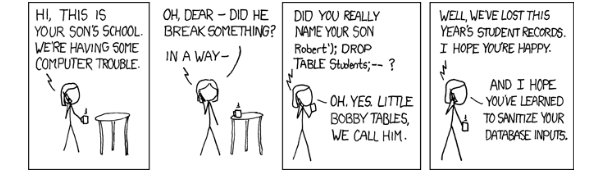
\includegraphics[width=1\textwidth]{sql-injection}
    \label{fig:LABEL}
\end{figure}


\textbf{Sanitize inputs!!} Use some libraries or other people functions in order to validate user inputs. But for what is SQL, we can use prepared statements. Use structured data with parameters and etc... (like with Spring Boot and SQL statements by giving string parameters)


To limit impact of SQL injections, \textcolor{red}{use different DB users different accesses}: 
\begin{itemize}
	\item One DB user with read access on the \verb|customer| table
		\begin{itemize}
			\item for login purposes
		\end{itemize}
	\item One DB user with write access on the \verb|customer| table
		\begin{itemize}
			\item for changing the users' password
		\end{itemize}
	\item One DB user with read access on the \verb|account| table
		\begin{itemize}
			\item customers can not change ownership of account
		\end{itemize}
	\item One DB user with read/write access to the transaction table
		\begin{itemize}
			\item for the actual application
		\end{itemize}
\end{itemize}

The database access control is not exactly least privilege, but it reduces the impact of SQL injection (and compartmentalizes code with privileges), e.g., an SQL injection on the login form cannot read data from the \verb|transaction| table

\begin{tcolorbox}[
  colback=orange!15,     % background color
  colframe=black!50,    % border color
  boxrule=1pt,       % border thickness
  arc=3mm,             % rounded corners
  left=4mm, right=4mm, top=2mm, bottom=2mm % padding
]
\textbf{What's missing for least privilege?}

\vspace{0.3cm}

We're still multiplexing all access on this single DB user. We're still missing the multitier (customers, database users, system administrator, server administrators, ...)

\end{tcolorbox}
\section*{Application Level Access Control}

Using different DB users is an application of the \textbf{defense in depth} principle

The application implements fine grained access control

The database implements coarse grained control

If the access control at the application level fails, the access control of the database reduces the impact. 

\textbf{Defense in depth}: multiple layers of security

\newpage

\begin{center}
  {\LARGE \textbf{Encrypting Data}}
\end{center}

\vspace{1cm}

% Quick centered image
\begin{figure}[H]
    \centering
    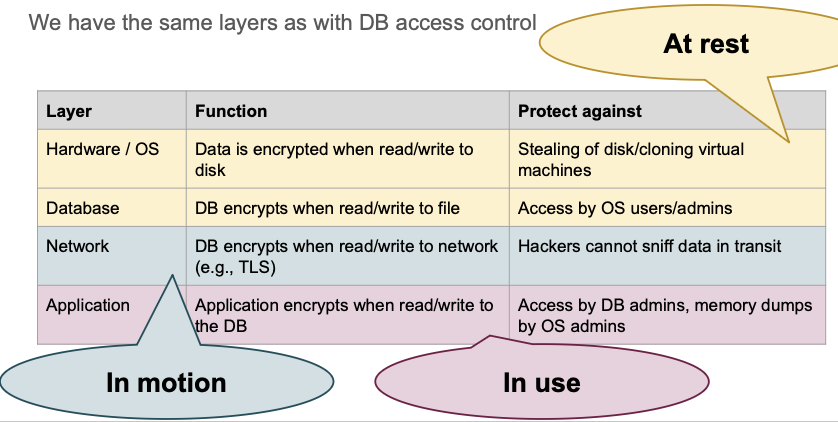
\includegraphics[width=0.8\textwidth]{encrypting-data}
    \label{fig:LABEL}
\end{figure}

\section*{Encrypting Data at Rest}

Data stored on the server is data at rest. The OS can encrypt the data before it is written to disks
\begin{itemize}
	\item Protects against theft/copy of the disks
	\item A user that can log into the machine and access the files of the database will see cleartext data!
\end{itemize}

Databases can be configured to encrypt data before writing it to files
\begin{itemize}
	\item File access by OS users does not yield cleartext data anymore
	\item The keys may be stored in local files or obtained from a key server, e.g., from the Amazon key management service for machines in the Amazon cloud
\end{itemize}

Most DBs call this type of encryption Transparent Data Encryption (TDE)

\textbf{Key use case}: Mobile phones!

\section*{Encrypting Data in Motion}

Data is exchanged between the DB and the application (web server or logic tier)

If not encrypted, it could be eavesdropped

Most DBs support TLS encryption for DB connections
\begin{itemize}
	\item Certificate pinning: the client (DB) can be given a copy of the server certificate or its CA
	\item It will refuse to connect if the server presents a different certificate (no need for 200 CAs as in web browsers)

\end{itemize}

For data centers, the bigger cost for encrypting data in motion is power consumption! 

\section*{Encrypting Data in Use by the Application}

With encryption at rest and in motion, data is still in clear in the memory of the DB!
\begin{itemize}
	\item AN admin of the DB server can dump the memory and see the data
\end{itemize}

The solution is to encrypt data in the application before storing it in the DB

The key stays in the application tier
\begin{itemize}
	\item There is no way to decrypt the data on the DB server
\end{itemize}

\begin{tcolorbox}[
  colback=gray!15,     % background color
  colframe=black!50,    % border color
  boxrule=1pt,       % border thickness
  arc=3mm,             % rounded corners
  left=4mm, right=4mm, top=2mm, bottom=2mm % padding
]
\textbf{Quiz: Encrypted Database}
What could go wrong if the data is encrypted in the database?
\vspace{0.3cm}

\textbf{Discussion}: We lose search capacities and sorting, compare or aggregating data. \\

This makes the DB pretty useless. But this is still useful for certain information:
\begin{itemize}
	\item Credit cards numbers
	\item Pin codes
	\item Passwords?
\end{itemize}
\end{tcolorbox}

\vspace{1cm}
\begin{center}
  {\LARGE \textbf{Password Storage}}
\end{center}

\vspace{1cm}

Password leaks are common...

On the darknet you can buy Terabytes of pairs of (username, password). 

\textbf{Site}: haveibeenpwned.com

\section*{Password Storage}

Naive approach: cleartext
\begin{itemize}
	\item You should \textbf{NEVER} store password in cleartext
\end{itemize}

Better: \textbf{hash} the password
\begin{itemize}
	\item Microsoft stores Windows passwords as hashes (MD4)
	\item (in MD4) Almost all passwords of length 8 can be recovered in under a minute
\end{itemize}

\section*{Password Storage: Hashing}

Classic way: use \textbf{salt} and \textbf{iterations} (to stop bruteforcing)
\begin{itemize}
	\item Hugely slows down password cracking
	\item Simple passwords can still be cracked on specialized hardware
\end{itemize}

Modern way: use a \textbf{memory hard} function

\begin{itemize}
	\item Cracking a password requires a decent amount of memory
	\item Specialized hardware with many computing cores do not have enough memory to speed-up cracking
\end{itemize}

\vspace{0.5cm}
\begin{center}
  {\LARGE \textbf{The Importance of Salt}}
\end{center}

SMBv1 (Microsoft) does not salt their passwords. Don't be like Microsoft.
\vspace{0.5cm}
\section*{Salt Usage and Examples}

Salt: Random data concatenated as an additional input to the hash function: \verb|pw_hash = h(password, salt)|

Examples
\begin{itemize}
	\item WPA and WPA2 use the SSID as salt, and 4,096 iterations of HMAC-SHA1
		\begin{itemize}
			\item Each test becomes expensive
			\item Only simple passwords can be cracked
		\end{itemize}
	\item Kerberos pre-authentication
\end{itemize}

\section*{The Importance of Salt}

Some systems store the passwords as a simple hash: \verb|pw_hash = h(password)|

If passwords are hashed without salt, there are two major weakness:

1. Multiple hashes can be cracked at once
\begin{itemize}
	\item If you have a list of 1,000 hashes and want to find out if any of the 1,000 accounts has password "correct horse battery staple";
		\begin{itemize}
			\item calculate \verb|h("correct horse battey staple")|
			\item look-up which of the 1,000 hashes matches
		\end{itemize}
	\item With a smart data structure, the look-up is almost free, with a single hash operation you can try to crack 1,000 passwords
	\item Cracking \textit{n} passwords requires the same hash operations as cracking one!

\end{itemize}


2. Hashes can be calculated in advance
\begin{itemize}
	\item Windows hashes have no salt
	\item If attackers had enough memory, they could calculate all hashes in advance and store them in a great big table
	\item The table would be about 4.7PB big! Not feasible
	\item Attackers can trade more time of cracking a password for a smaller table
\end{itemize}


\section*{Time-Memory Trade-Offs (TMTO)}

In 1980 Martin Hellman invented a TMTO to inverse cryptographic functions

\begin{itemize}
	\item When you double the memory, it is four times faster to invert the function
\end{itemize}

% Quick centered image
\begin{figure}[H]
    \centering
    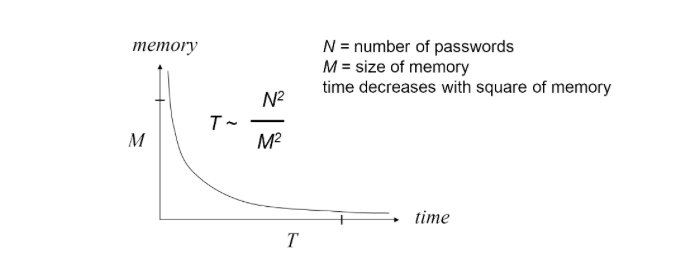
\includegraphics[width=0.7\textwidth]{TMTO}
    \label{fig:LABEL}
\end{figure}

\textbf{Rainbow Tables} are an optimization of this TMTO from 2003

\section*{Password Cracking: Time-Memory Trade-Offs}

Basic idea: Trade \underline{more time of cracking a password} for \underline{a smaller table}

Originally, we can crack one password from one password-hash pair
\begin{itemize}
	\item Number of passwords: \verb|n|
	\item Memory required: \verb|n * (password_len + hash_len)|
	\item Time of cracking password: \verb|time of finding a hash match, i.e., O(c)|
\end{itemize}

Can we crack two passwords from one password-hash pair?
\begin{itemize}
	\item Number of passwords: \verb|n|
	\item Memory required": \verb|1/2 * n * (password_len + hash_len)|
\end{itemize}
How can we connect the two password-hash pairs?
\begin{itemize}
	\item Reduction function (\textbf{magic function})
	\item Map from the hash set to the password set
\end{itemize}

\begin{tcolorbox}[
  colback=gray!15,     % background color
  colframe=black!50,    % border color
  boxrule=1pt,       % border thickness
  arc=3mm,             % rounded corners
  left=4mm, right=4mm, top=2mm, bottom=2mm % padding
]
\textbf{Quiz: Password Cracking}
What makes a good reduction function? 
\vspace{0.3cm}

The reduction function glues the hash of the previous computation to the current one. \\

Requirements:
\begin{itemize}
	\item Few collisions
	\item Output follows the expected alphabet
	\item Output is reasonably uniformly distributed
	\item Does NOT require any specific structure
\end{itemize}

\end{tcolorbox}

Main idea: reduce memory by half and use computer power with the reduction function to find informations!

More columns, more time of cracking a password, less memory consumption. 
Typically, chains would contain tens of thousands of hashes and passwords. 

% Quick centered image
\begin{figure}[H]
    \centering
    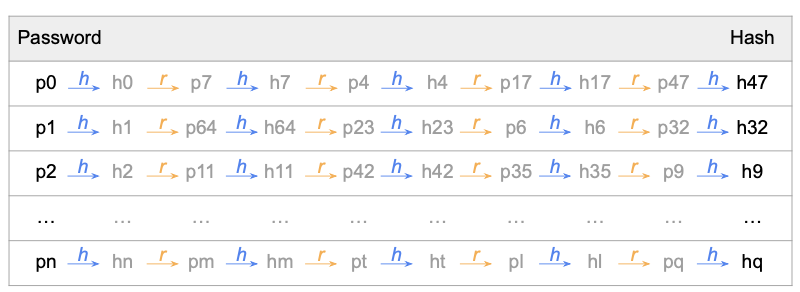
\includegraphics[width=0.7\textwidth]{password-cracking-table}
    \label{fig:LABEL}
\end{figure}

Challenge: Reduction function may collide. 

Result in identical chains, which is a waste of table space. 

\section*{Password Cracking: Rainbow table}

Solution: Using a different reduction function in each column of the table

This allows building much larger tables and makes them much more efficient. 

% Quick centered image
\begin{figure}[H]
    \centering
    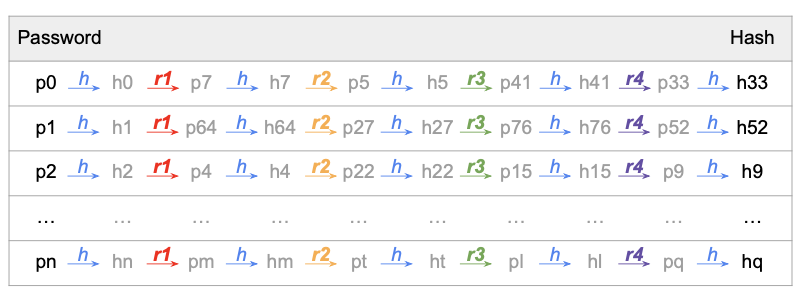
\includegraphics[width=0.7\textwidth]{rainbow}
    \label{fig:LABEL}
\end{figure}

\newpage

\begin{center}
  {\LARGE \textbf{Storing Hashes with Salt and Iterations}} \\
  The classical way
\end{center}

\vspace{1cm}

\section*{Using Salt}

Adding a random value (\textbf{salt}) to the hash function prevents the two issues: 
\begin{itemize}
	\item You cannot crack multiple hashes with a single hash calculation
	\item You cannot calculate the hashes in advance
\end{itemize}

Because each has a different, random salt
\begin{center}
	\verb|salt = random()| \\
	\verb|pw_hash = h(password, salt)|
\end{center}

We need to store both the hast and the salt in the database
\begin{itemize}
	\item When a user logs in, we use the salt to generate a hash and compare it to the stored hash
\end{itemize}

\begin{tcolorbox}[
  colback=gray!15,     % background color
  colframe=black!50,    % border color
  boxrule=1pt,       % border thickness
  arc=3mm,             % rounded corners
  left=4mm, right=4mm, top=2mm, bottom=2mm % padding
]
\textbf{Quiz!} \\
What cryptographic primitive can we use to combine a salt with a hash? \\
How can we make it harder to crack? \\

\vspace{0.5cm}
Cryptographic hash functions are used to hash passwords and salt \\

They are repeated many times to make it harder to crack
\end{tcolorbox}

\section*{Salt Is Not Enough}

Cryptographic hash functions are designed to be fast and simple to implement

A modern graphics card calculates hundreds of billions of hashes per second

A simple way of slowing the attacker is to apply the hash function multiple times

If you require 5,000 iterations for creating the password hash
\begin{itemize}
	\item Login will take 5,000 times longer (e.g., 0.05s instead of 0.00001s)
	\item Cracking will be 5,000 times slower (e.g., 2 years instead of 4 hours)
\end{itemize}

\section*{Salt and Iterations: Standards}

There is an official standard for using salt and iterations in hash functions. 

The current version is Password Based Key Derivation Function 2 (PBKDF2, RFC 8018)

Used for example in
\begin{itemize}
	\item Wi-Fi WPA
	\item MacOS user password hashes
	\item Linux disk encryption (LUKS)
	\item Previously for Linux passwords (SHA512, 5000 iterations)
\end{itemize}

\vspace{1cm}

\begin{center}
  {\LARGE \textbf{Memory Hard Hash Function}} \\
  The modern way of hashing passwords
\end{center}

\vspace{1cm}

\section*{Memory Hard Functions}

Iterating a cryptographic hash function is not the best way to slow down an attacker

Specialized hardware (graphics cards, FPGAs) computers tera-hashes in parallel
\begin{itemize}
	\item E.g., it takes less than 50k transistors to implement SHA512
\end{itemize}
Better password hash functions require a certain amount of memory (e.g., 16MB)
\begin{itemize}
	\item For a single login operation, 16MB are easily available
	\item Graphics cards or FPGAs would need gigabytes of internal memory to parallelize thousands of hashes
	\item E.g., it takes millions of transistors to store 16MB of data
\end{itemize}

The functions run through many steps and intermediate results are stored in memory. Since each step depends on result from previous steps, if you do not have enough memory you can still calculate the result
\begin{itemize}
	\item Buy you have to recalculate intermediate values again and again
\end{itemize}

Typical memory hard hash functions can be parameterized:
\begin{itemize}
	\item Choose the amount of memory needed
	\item Choose the number of steps to calculate
\end{itemize}
\textbf{When implementing password storage}

\begin{itemize}
	\item Always use salt and make the hash function slow
	\item USe Yescrypt, Scrypt, or Argon2 if available
	\item If not, use PBKDF2
\end{itemize}

Most \textbf{Linux} distributions switched to yescrypt 

\section*{Summary of Password Storage}
\textbf{NEVER} store passwords in cleartext

Always use \textbf{salt} to store passwords. If you do not:
\begin{itemize}
	\item Multiple hashes can be cracked at once
	\item Hashes can be calculated in advance
		\begin{itemize}
			\item Rainbow tables efficiently store this information
		\end{itemize}
\end{itemize}

Salt is insufficient, must slow down hash function
\begin{itemize}
	\item Iterations are a good start
		\begin{itemize}
			\item PBKDF2 is the standard way of doing it
		\end{itemize}
	\item Memory hard functions are better
		\begin{itemize}
			\item They are more expensive to parallelize (GPUs and FPGAs have little internal memory)
			\item Examples: Yescrypt, Scrypt, or Argon2
		\end{itemize}
\end{itemize}

\vspace{0.5cm}
\begin{center}
  {\LARGE \textbf{Secure Remote Password Protocol (SRP)}}
\end{center}

\vspace{1cm}

\section*{Introduction}

Secure Remote Password protocol (SRP): A Password Authenticated Key Exchange (PAKE)

A PAKE allows to 
\begin{itemize}
	\item Verify the password of a remote party
	\item Exchange a key (e.g., for encryption)
\end{itemize}

In TLS, the server can sign its half of the Diffie Hellman key exchange to prove possession of the private key of the certificate, thus proving its identity

% Quick centered image
\begin{figure}[H]
    \centering
    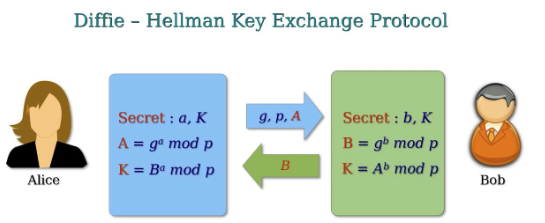
\includegraphics[width=0.8\textwidth]{dh}
    \label{fig:LABEL}
\end{figure}

PAKE is similar (based on Diffie Hellman), but authentication is based on the password as key where the server stores information "about" the password

It can't be cracked, even if the attacker sees all messages.

\newpage

\section*{SRP Overview}

SRP is like DH with additional elements that depend on the password

It uses exponentiations of a generator \verb|g| (e.g., $g^{k}$) and a modulo \textit{N}

For each user, the server stores three elements:

1. The username \textit{U}
2. A salt \textit{s}
3. The password verifier \textit{v} (the exponentiation of a salted hash of the password \textit{p}):"

% Quick centered image
\begin{figure}[H]
    \centering
    \includegraphics[width=0.7\textwidth]{SRP}
    \label{fig:LABEL}
\end{figure}

The server adds \textit{v} to its part of the Diffie-Hellman exchange
\begin{itemize}
	\item It contributes to the calculation of the key
\end{itemize}

The client will need to know the salt to calculate \textit{x}, so it first asks for this

% Quick centered image
\begin{figure}[H]
    \centering
    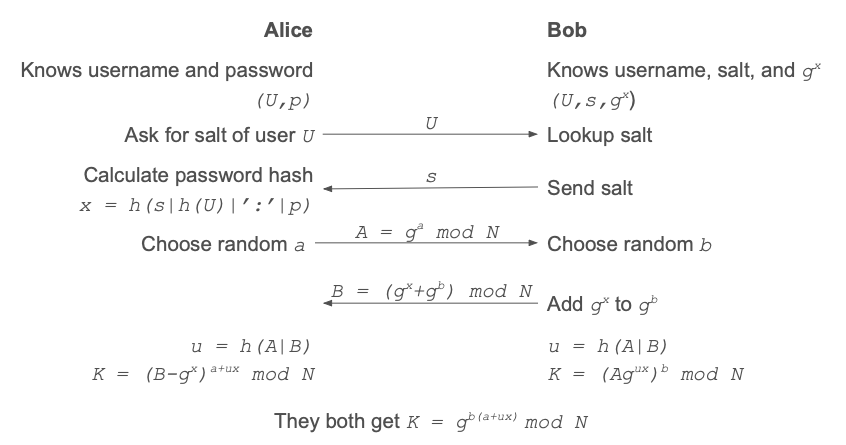
\includegraphics[width=0.8\textwidth]{srp-diagram}
    \label{fig:LABEL}
\end{figure}

\section*{SRP summary}

Alice and Bob have only exchange public values: $g^{a}$ and $g^{b} + g^{x}$ 

Eavesdropper cannot learn anything from these values
\begin{itemize}
	\item In particular: they cannot brute-fore the password
\end{itemize}

The resulting key depends on \textit{a, b} \verb|and| \textit{x} (\textit{x} depends on the password)

Bob only knows the public value $g^{x}$ 

\begin{itemize}
	\item If a hacker takes control of Bob, they do not learn the password hash \textit{x}
	\item They could try to brute force the password from $g^{x}$
\end{itemize}
Before continuing, they can send each other an encrypted message or a MAC to prove that they succeeded in calculating the key.
\end{document}
